% Graphic for TeX using PGF
% Title: C:\Users\Kaylen\CotWM\Doc\UML\AI_Combat.dia
% Creator: Dia v0.97.1
% CreationDate: Sun Mar 11 15:41:22 2012
% For: Kaylen
% \usepackage{tikz}
% The following commands are not supported in PSTricks at present
% We define them conditionally, so when they are implemented,
% this pgf file will use them.
\ifx\du\undefined
  \newlength{\du}
\fi
\setlength{\du}{15\unitlength}
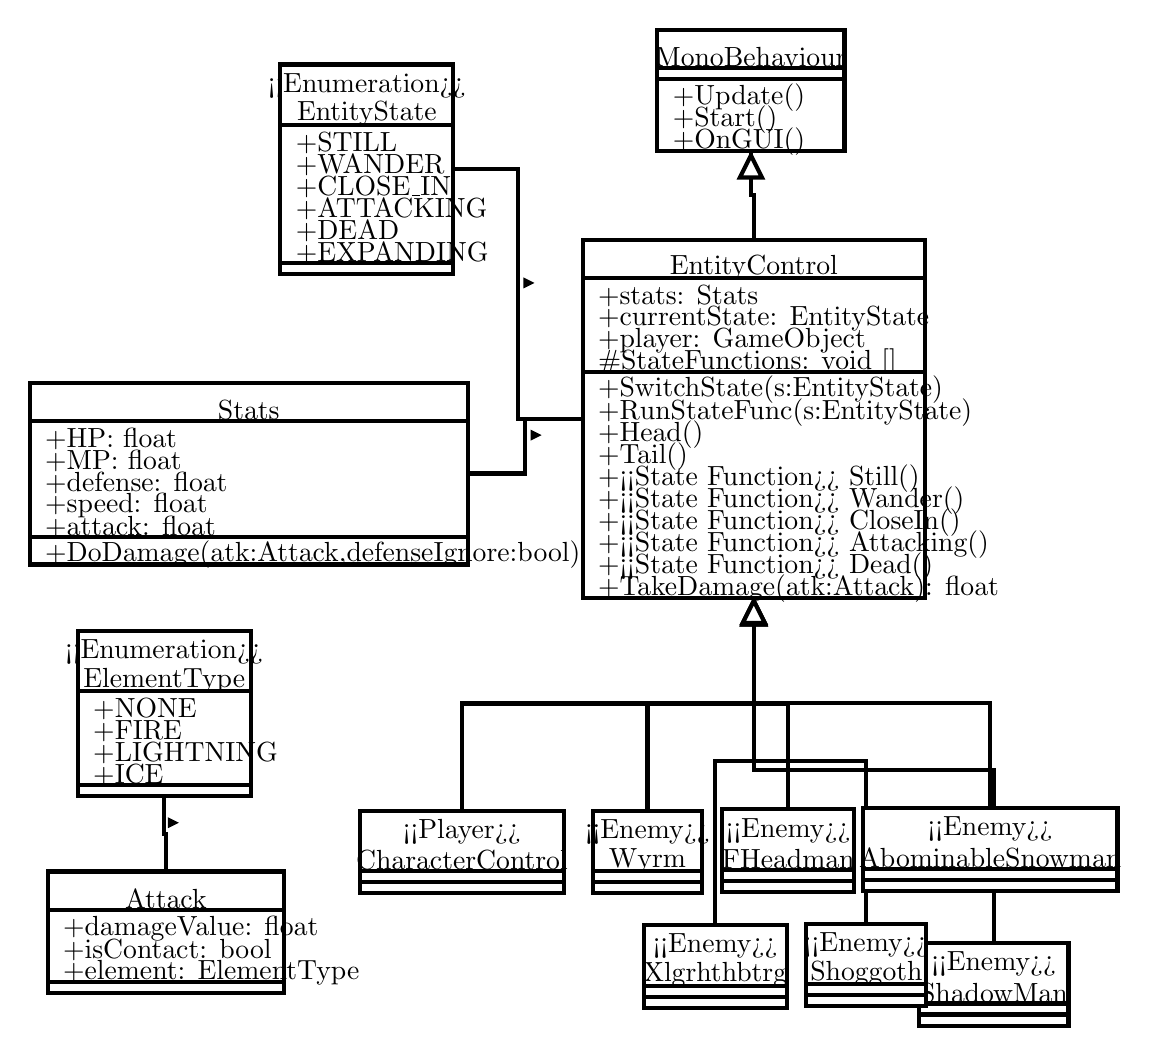
\begin{tikzpicture}
\pgftransformxscale{0.663512}
\pgftransformyscale{-0.663512}
\definecolor{dialinecolor}{rgb}{0.000000, 0.000000, 0.000000}
\pgfsetstrokecolor{dialinecolor}
\definecolor{dialinecolor}{rgb}{1.000000, 1.000000, 1.000000}
\pgfsetfillcolor{dialinecolor}
\pgfsetlinewidth{0.100000\du}
\pgfsetdash{}{0pt}
\definecolor{dialinecolor}{rgb}{1.000000, 1.000000, 1.000000}
\pgfsetfillcolor{dialinecolor}
\fill (-6.800000\du,4.250000\du)--(-6.800000\du,5.650000\du)--(5.635000\du,5.650000\du)--(5.635000\du,4.250000\du)--cycle;
\definecolor{dialinecolor}{rgb}{0.000000, 0.000000, 0.000000}
\pgfsetstrokecolor{dialinecolor}
\draw (-6.800000\du,4.250000\du)--(-6.800000\du,5.650000\du)--(5.635000\du,5.650000\du)--(5.635000\du,4.250000\du)--cycle;
% setfont left to latex
\definecolor{dialinecolor}{rgb}{0.000000, 0.000000, 0.000000}
\pgfsetstrokecolor{dialinecolor}
\node at (-0.582500\du,5.250000\du){EntityControl};
\definecolor{dialinecolor}{rgb}{1.000000, 1.000000, 1.000000}
\pgfsetfillcolor{dialinecolor}
\fill (-6.800000\du,5.650000\du)--(-6.800000\du,9.050000\du)--(5.635000\du,9.050000\du)--(5.635000\du,5.650000\du)--cycle;
\definecolor{dialinecolor}{rgb}{0.000000, 0.000000, 0.000000}
\pgfsetstrokecolor{dialinecolor}
\draw (-6.800000\du,5.650000\du)--(-6.800000\du,9.050000\du)--(5.635000\du,9.050000\du)--(5.635000\du,5.650000\du)--cycle;
% setfont left to latex
\definecolor{dialinecolor}{rgb}{0.000000, 0.000000, 0.000000}
\pgfsetstrokecolor{dialinecolor}
\node[anchor=west] at (-6.650000\du,6.310000\du){+stats: Stats};
% setfont left to latex
\definecolor{dialinecolor}{rgb}{0.000000, 0.000000, 0.000000}
\pgfsetstrokecolor{dialinecolor}
\node[anchor=west] at (-6.650000\du,7.110000\du){+currentState: EntityState};
% setfont left to latex
\definecolor{dialinecolor}{rgb}{0.000000, 0.000000, 0.000000}
\pgfsetstrokecolor{dialinecolor}
\node[anchor=west] at (-6.650000\du,7.910000\du){+player: GameObject};
% setfont left to latex
\definecolor{dialinecolor}{rgb}{0.000000, 0.000000, 0.000000}
\pgfsetstrokecolor{dialinecolor}
\node[anchor=west] at (-6.650000\du,8.710000\du){\#StateFunctions: void \ensuremath{[}\ensuremath{]}};
\definecolor{dialinecolor}{rgb}{1.000000, 1.000000, 1.000000}
\pgfsetfillcolor{dialinecolor}
\fill (-6.800000\du,9.050000\du)--(-6.800000\du,17.250000\du)--(5.635000\du,17.250000\du)--(5.635000\du,9.050000\du)--cycle;
\definecolor{dialinecolor}{rgb}{0.000000, 0.000000, 0.000000}
\pgfsetstrokecolor{dialinecolor}
\draw (-6.800000\du,9.050000\du)--(-6.800000\du,17.250000\du)--(5.635000\du,17.250000\du)--(5.635000\du,9.050000\du)--cycle;
% setfont left to latex
\definecolor{dialinecolor}{rgb}{0.000000, 0.000000, 0.000000}
\pgfsetstrokecolor{dialinecolor}
\node[anchor=west] at (-6.650000\du,9.710000\du){+SwitchState(s:EntityState)};
% setfont left to latex
\definecolor{dialinecolor}{rgb}{0.000000, 0.000000, 0.000000}
\pgfsetstrokecolor{dialinecolor}
\node[anchor=west] at (-6.650000\du,10.510000\du){+RunStateFunc(s:EntityState)};
% setfont left to latex
\definecolor{dialinecolor}{rgb}{0.000000, 0.000000, 0.000000}
\pgfsetstrokecolor{dialinecolor}
\node[anchor=west] at (-6.650000\du,11.310000\du){+Head()};
% setfont left to latex
\definecolor{dialinecolor}{rgb}{0.000000, 0.000000, 0.000000}
\pgfsetstrokecolor{dialinecolor}
\node[anchor=west] at (-6.650000\du,12.110000\du){+Tail()};
% setfont left to latex
\definecolor{dialinecolor}{rgb}{0.000000, 0.000000, 0.000000}
\pgfsetstrokecolor{dialinecolor}
\node[anchor=west] at (-6.650000\du,12.910000\du){+<<State Function>> Still()};
% setfont left to latex
\definecolor{dialinecolor}{rgb}{0.000000, 0.000000, 0.000000}
\pgfsetstrokecolor{dialinecolor}
\node[anchor=west] at (-6.650000\du,13.710000\du){+<<State Function>> Wander()};
% setfont left to latex
\definecolor{dialinecolor}{rgb}{0.000000, 0.000000, 0.000000}
\pgfsetstrokecolor{dialinecolor}
\node[anchor=west] at (-6.650000\du,14.510000\du){+<<State Function>> CloseIn()};
% setfont left to latex
\definecolor{dialinecolor}{rgb}{0.000000, 0.000000, 0.000000}
\pgfsetstrokecolor{dialinecolor}
\node[anchor=west] at (-6.650000\du,15.310000\du){+<<State Function>> Attacking()};
% setfont left to latex
\definecolor{dialinecolor}{rgb}{0.000000, 0.000000, 0.000000}
\pgfsetstrokecolor{dialinecolor}
\node[anchor=west] at (-6.650000\du,16.110000\du){+<<State Function>> Dead()};
% setfont left to latex
\definecolor{dialinecolor}{rgb}{0.000000, 0.000000, 0.000000}
\pgfsetstrokecolor{dialinecolor}
\node[anchor=west] at (-6.650000\du,16.910000\du){+TakeDamage(atk:Attack): float};
\pgfsetlinewidth{0.100000\du}
\pgfsetdash{}{0pt}
\definecolor{dialinecolor}{rgb}{1.000000, 1.000000, 1.000000}
\pgfsetfillcolor{dialinecolor}
\fill (-4.084280\du,-3.371880\du)--(-4.084280\du,-1.971880\du)--(2.710720\du,-1.971880\du)--(2.710720\du,-3.371880\du)--cycle;
\definecolor{dialinecolor}{rgb}{0.000000, 0.000000, 0.000000}
\pgfsetstrokecolor{dialinecolor}
\draw (-4.084280\du,-3.371880\du)--(-4.084280\du,-1.971880\du)--(2.710720\du,-1.971880\du)--(2.710720\du,-3.371880\du)--cycle;
% setfont left to latex
\definecolor{dialinecolor}{rgb}{0.000000, 0.000000, 0.000000}
\pgfsetstrokecolor{dialinecolor}
\node at (-0.686780\du,-2.371880\du){MonoBehaviour};
\definecolor{dialinecolor}{rgb}{1.000000, 1.000000, 1.000000}
\pgfsetfillcolor{dialinecolor}
\fill (-4.084280\du,-1.971880\du)--(-4.084280\du,-1.571880\du)--(2.710720\du,-1.571880\du)--(2.710720\du,-1.971880\du)--cycle;
\definecolor{dialinecolor}{rgb}{0.000000, 0.000000, 0.000000}
\pgfsetstrokecolor{dialinecolor}
\draw (-4.084280\du,-1.971880\du)--(-4.084280\du,-1.571880\du)--(2.710720\du,-1.571880\du)--(2.710720\du,-1.971880\du)--cycle;
\definecolor{dialinecolor}{rgb}{1.000000, 1.000000, 1.000000}
\pgfsetfillcolor{dialinecolor}
\fill (-4.084280\du,-1.571880\du)--(-4.084280\du,1.028120\du)--(2.710720\du,1.028120\du)--(2.710720\du,-1.571880\du)--cycle;
\definecolor{dialinecolor}{rgb}{0.000000, 0.000000, 0.000000}
\pgfsetstrokecolor{dialinecolor}
\draw (-4.084280\du,-1.571880\du)--(-4.084280\du,1.028120\du)--(2.710720\du,1.028120\du)--(2.710720\du,-1.571880\du)--cycle;
% setfont left to latex
\definecolor{dialinecolor}{rgb}{0.000000, 0.000000, 0.000000}
\pgfsetstrokecolor{dialinecolor}
\node[anchor=west] at (-3.934280\du,-0.911880\du){+Update()};
% setfont left to latex
\definecolor{dialinecolor}{rgb}{0.000000, 0.000000, 0.000000}
\pgfsetstrokecolor{dialinecolor}
\node[anchor=west] at (-3.934280\du,-0.111880\du){+Start()};
% setfont left to latex
\definecolor{dialinecolor}{rgb}{0.000000, 0.000000, 0.000000}
\pgfsetstrokecolor{dialinecolor}
\node[anchor=west] at (-3.934280\du,0.688120\du){+OnGUI()};
\pgfsetlinewidth{0.100000\du}
\pgfsetdash{}{0pt}
\pgfsetmiterjoin
\pgfsetbuttcap
{
\definecolor{dialinecolor}{rgb}{0.000000, 0.000000, 0.000000}
\pgfsetfillcolor{dialinecolor}
% was here!!!
\definecolor{dialinecolor}{rgb}{0.000000, 0.000000, 0.000000}
\pgfsetstrokecolor{dialinecolor}
\draw (-0.686780\du,1.078395\du)--(-0.686780\du,2.638997\du)--(-0.582500\du,2.638997\du)--(-0.582500\du,4.199600\du);
}
\definecolor{dialinecolor}{rgb}{0.000000, 0.000000, 0.000000}
\pgfsetstrokecolor{dialinecolor}
\draw (-0.686780\du,1.990198\du)--(-0.686780\du,2.638997\du)--(-0.582500\du,2.638997\du)--(-0.582500\du,4.199600\du);
\pgfsetmiterjoin
\definecolor{dialinecolor}{rgb}{1.000000, 1.000000, 1.000000}
\pgfsetfillcolor{dialinecolor}
\fill (-0.286780\du,1.990198\du)--(-0.686780\du,1.190198\du)--(-1.086780\du,1.990198\du)--cycle;
\pgfsetlinewidth{0.100000\du}
\pgfsetdash{}{0pt}
\pgfsetmiterjoin
\definecolor{dialinecolor}{rgb}{0.000000, 0.000000, 0.000000}
\pgfsetstrokecolor{dialinecolor}
\draw (-0.286780\du,1.990198\du)--(-0.686780\du,1.190198\du)--(-1.086780\du,1.990198\du)--cycle;
% setfont left to latex
\pgfsetlinewidth{0.100000\du}
\pgfsetdash{}{0pt}
\definecolor{dialinecolor}{rgb}{1.000000, 1.000000, 1.000000}
\pgfsetfillcolor{dialinecolor}
\fill (-17.771800\du,-2.109380\du)--(-17.771800\du,0.090620\du)--(-11.496800\du,0.090620\du)--(-11.496800\du,-2.109380\du)--cycle;
\definecolor{dialinecolor}{rgb}{0.000000, 0.000000, 0.000000}
\pgfsetstrokecolor{dialinecolor}
\draw (-17.771800\du,-2.109380\du)--(-17.771800\du,0.090620\du)--(-11.496800\du,0.090620\du)--(-11.496800\du,-2.109380\du)--cycle;
% setfont left to latex
\definecolor{dialinecolor}{rgb}{0.000000, 0.000000, 0.000000}
\pgfsetstrokecolor{dialinecolor}
\node at (-14.634300\du,-1.349380\du){<<Enumeration>>};
% setfont left to latex
\definecolor{dialinecolor}{rgb}{0.000000, 0.000000, 0.000000}
\pgfsetstrokecolor{dialinecolor}
\node at (-14.634300\du,-0.309380\du){EntityState};
\definecolor{dialinecolor}{rgb}{1.000000, 1.000000, 1.000000}
\pgfsetfillcolor{dialinecolor}
\fill (-17.771800\du,0.090620\du)--(-17.771800\du,5.090620\du)--(-11.496800\du,5.090620\du)--(-11.496800\du,0.090620\du)--cycle;
\definecolor{dialinecolor}{rgb}{0.000000, 0.000000, 0.000000}
\pgfsetstrokecolor{dialinecolor}
\draw (-17.771800\du,0.090620\du)--(-17.771800\du,5.090620\du)--(-11.496800\du,5.090620\du)--(-11.496800\du,0.090620\du)--cycle;
% setfont left to latex
\definecolor{dialinecolor}{rgb}{0.000000, 0.000000, 0.000000}
\pgfsetstrokecolor{dialinecolor}
\node[anchor=west] at (-17.621800\du,0.750620\du){+STILL};
% setfont left to latex
\definecolor{dialinecolor}{rgb}{0.000000, 0.000000, 0.000000}
\pgfsetstrokecolor{dialinecolor}
\node[anchor=west] at (-17.621800\du,1.550620\du){+WANDER};
% setfont left to latex
\definecolor{dialinecolor}{rgb}{0.000000, 0.000000, 0.000000}
\pgfsetstrokecolor{dialinecolor}
\node[anchor=west] at (-17.621800\du,2.350620\du){+CLOSE\_IN};
% setfont left to latex
\definecolor{dialinecolor}{rgb}{0.000000, 0.000000, 0.000000}
\pgfsetstrokecolor{dialinecolor}
\node[anchor=west] at (-17.621800\du,3.150620\du){+ATTACKING};
% setfont left to latex
\definecolor{dialinecolor}{rgb}{0.000000, 0.000000, 0.000000}
\pgfsetstrokecolor{dialinecolor}
\node[anchor=west] at (-17.621800\du,3.950620\du){+DEAD};
% setfont left to latex
\definecolor{dialinecolor}{rgb}{0.000000, 0.000000, 0.000000}
\pgfsetstrokecolor{dialinecolor}
\node[anchor=west] at (-17.621800\du,4.750620\du){+EXPANDING};
\definecolor{dialinecolor}{rgb}{1.000000, 1.000000, 1.000000}
\pgfsetfillcolor{dialinecolor}
\fill (-17.771800\du,5.090620\du)--(-17.771800\du,5.490620\du)--(-11.496800\du,5.490620\du)--(-11.496800\du,5.090620\du)--cycle;
\definecolor{dialinecolor}{rgb}{0.000000, 0.000000, 0.000000}
\pgfsetstrokecolor{dialinecolor}
\draw (-17.771800\du,5.090620\du)--(-17.771800\du,5.490620\du)--(-11.496800\du,5.490620\du)--(-11.496800\du,5.090620\du)--cycle;
\pgfsetlinewidth{0.100000\du}
\pgfsetdash{}{0pt}
\pgfsetmiterjoin
\pgfsetbuttcap
{
\definecolor{dialinecolor}{rgb}{0.000000, 0.000000, 0.000000}
\pgfsetfillcolor{dialinecolor}
% was here!!!
\definecolor{dialinecolor}{rgb}{0.000000, 0.000000, 0.000000}
\pgfsetstrokecolor{dialinecolor}
\draw (-11.446411\du,1.690620\du)--(-9.148397\du,1.690620\du)--(-9.148397\du,10.750000\du)--(-6.850383\du,10.750000\du);
}
% setfont left to latex
\definecolor{dialinecolor}{rgb}{0.000000, 0.000000, 0.000000}
\pgfsetstrokecolor{dialinecolor}
\node[anchor=west] at (-9.048397\du,6.020310\du){};
\definecolor{dialinecolor}{rgb}{0.000000, 0.000000, 0.000000}
\pgfsetfillcolor{dialinecolor}
\fill (-8.948397\du,6.020310\du)--(-8.948397\du,5.620310\du)--(-8.548397\du,5.820310\du)--cycle;
\definecolor{dialinecolor}{rgb}{0.000000, 0.000000, 0.000000}
\pgfsetstrokecolor{dialinecolor}
\node[anchor=west] at (-11.246411\du,1.490620\du){};
\definecolor{dialinecolor}{rgb}{0.000000, 0.000000, 0.000000}
\pgfsetstrokecolor{dialinecolor}
\node[anchor=east] at (-7.050383\du,10.550000\du){};
\pgfsetlinewidth{0.100000\du}
\pgfsetdash{}{0pt}
\definecolor{dialinecolor}{rgb}{1.000000, 1.000000, 1.000000}
\pgfsetfillcolor{dialinecolor}
\fill (-26.871800\du,9.440620\du)--(-26.871800\du,10.840620\du)--(-10.971800\du,10.840620\du)--(-10.971800\du,9.440620\du)--cycle;
\definecolor{dialinecolor}{rgb}{0.000000, 0.000000, 0.000000}
\pgfsetstrokecolor{dialinecolor}
\draw (-26.871800\du,9.440620\du)--(-26.871800\du,10.840620\du)--(-10.971800\du,10.840620\du)--(-10.971800\du,9.440620\du)--cycle;
% setfont left to latex
\definecolor{dialinecolor}{rgb}{0.000000, 0.000000, 0.000000}
\pgfsetstrokecolor{dialinecolor}
\node at (-18.921800\du,10.440620\du){Stats};
\definecolor{dialinecolor}{rgb}{1.000000, 1.000000, 1.000000}
\pgfsetfillcolor{dialinecolor}
\fill (-26.871800\du,10.840620\du)--(-26.871800\du,15.040620\du)--(-10.971800\du,15.040620\du)--(-10.971800\du,10.840620\du)--cycle;
\definecolor{dialinecolor}{rgb}{0.000000, 0.000000, 0.000000}
\pgfsetstrokecolor{dialinecolor}
\draw (-26.871800\du,10.840620\du)--(-26.871800\du,15.040620\du)--(-10.971800\du,15.040620\du)--(-10.971800\du,10.840620\du)--cycle;
% setfont left to latex
\definecolor{dialinecolor}{rgb}{0.000000, 0.000000, 0.000000}
\pgfsetstrokecolor{dialinecolor}
\node[anchor=west] at (-26.721800\du,11.500620\du){+HP: float};
% setfont left to latex
\definecolor{dialinecolor}{rgb}{0.000000, 0.000000, 0.000000}
\pgfsetstrokecolor{dialinecolor}
\node[anchor=west] at (-26.721800\du,12.300620\du){+MP: float};
% setfont left to latex
\definecolor{dialinecolor}{rgb}{0.000000, 0.000000, 0.000000}
\pgfsetstrokecolor{dialinecolor}
\node[anchor=west] at (-26.721800\du,13.100620\du){+defense: float};
% setfont left to latex
\definecolor{dialinecolor}{rgb}{0.000000, 0.000000, 0.000000}
\pgfsetstrokecolor{dialinecolor}
\node[anchor=west] at (-26.721800\du,13.900620\du){+speed: float};
% setfont left to latex
\definecolor{dialinecolor}{rgb}{0.000000, 0.000000, 0.000000}
\pgfsetstrokecolor{dialinecolor}
\node[anchor=west] at (-26.721800\du,14.700620\du){+attack: float};
\definecolor{dialinecolor}{rgb}{1.000000, 1.000000, 1.000000}
\pgfsetfillcolor{dialinecolor}
\fill (-26.871800\du,15.040620\du)--(-26.871800\du,16.040620\du)--(-10.971800\du,16.040620\du)--(-10.971800\du,15.040620\du)--cycle;
\definecolor{dialinecolor}{rgb}{0.000000, 0.000000, 0.000000}
\pgfsetstrokecolor{dialinecolor}
\draw (-26.871800\du,15.040620\du)--(-26.871800\du,16.040620\du)--(-10.971800\du,16.040620\du)--(-10.971800\du,15.040620\du)--cycle;
% setfont left to latex
\definecolor{dialinecolor}{rgb}{0.000000, 0.000000, 0.000000}
\pgfsetstrokecolor{dialinecolor}
\node[anchor=west] at (-26.721800\du,15.700620\du){+DoDamage(atk:Attack,defenseIgnore:bool)};
\pgfsetlinewidth{0.100000\du}
\pgfsetdash{}{0pt}
\definecolor{dialinecolor}{rgb}{1.000000, 1.000000, 1.000000}
\pgfsetfillcolor{dialinecolor}
\fill (-26.221800\du,27.190600\du)--(-26.221800\du,28.590600\du)--(-17.636800\du,28.590600\du)--(-17.636800\du,27.190600\du)--cycle;
\definecolor{dialinecolor}{rgb}{0.000000, 0.000000, 0.000000}
\pgfsetstrokecolor{dialinecolor}
\draw (-26.221800\du,27.190600\du)--(-26.221800\du,28.590600\du)--(-17.636800\du,28.590600\du)--(-17.636800\du,27.190600\du)--cycle;
% setfont left to latex
\definecolor{dialinecolor}{rgb}{0.000000, 0.000000, 0.000000}
\pgfsetstrokecolor{dialinecolor}
\node at (-21.929300\du,28.190600\du){Attack};
\definecolor{dialinecolor}{rgb}{1.000000, 1.000000, 1.000000}
\pgfsetfillcolor{dialinecolor}
\fill (-26.221800\du,28.590600\du)--(-26.221800\du,31.190600\du)--(-17.636800\du,31.190600\du)--(-17.636800\du,28.590600\du)--cycle;
\definecolor{dialinecolor}{rgb}{0.000000, 0.000000, 0.000000}
\pgfsetstrokecolor{dialinecolor}
\draw (-26.221800\du,28.590600\du)--(-26.221800\du,31.190600\du)--(-17.636800\du,31.190600\du)--(-17.636800\du,28.590600\du)--cycle;
% setfont left to latex
\definecolor{dialinecolor}{rgb}{0.000000, 0.000000, 0.000000}
\pgfsetstrokecolor{dialinecolor}
\node[anchor=west] at (-26.071800\du,29.250600\du){+damageValue: float};
% setfont left to latex
\definecolor{dialinecolor}{rgb}{0.000000, 0.000000, 0.000000}
\pgfsetstrokecolor{dialinecolor}
\node[anchor=west] at (-26.071800\du,30.050600\du){+isContact: bool};
% setfont left to latex
\definecolor{dialinecolor}{rgb}{0.000000, 0.000000, 0.000000}
\pgfsetstrokecolor{dialinecolor}
\node[anchor=west] at (-26.071800\du,30.850600\du){+element: ElementType};
\definecolor{dialinecolor}{rgb}{1.000000, 1.000000, 1.000000}
\pgfsetfillcolor{dialinecolor}
\fill (-26.221800\du,31.190600\du)--(-26.221800\du,31.590600\du)--(-17.636800\du,31.590600\du)--(-17.636800\du,31.190600\du)--cycle;
\definecolor{dialinecolor}{rgb}{0.000000, 0.000000, 0.000000}
\pgfsetstrokecolor{dialinecolor}
\draw (-26.221800\du,31.190600\du)--(-26.221800\du,31.590600\du)--(-17.636800\du,31.590600\du)--(-17.636800\du,31.190600\du)--cycle;
\pgfsetlinewidth{0.100000\du}
\pgfsetdash{}{0pt}
\definecolor{dialinecolor}{rgb}{1.000000, 1.000000, 1.000000}
\pgfsetfillcolor{dialinecolor}
\fill (-25.126800\du,18.445600\du)--(-25.126800\du,20.645600\du)--(-18.851800\du,20.645600\du)--(-18.851800\du,18.445600\du)--cycle;
\definecolor{dialinecolor}{rgb}{0.000000, 0.000000, 0.000000}
\pgfsetstrokecolor{dialinecolor}
\draw (-25.126800\du,18.445600\du)--(-25.126800\du,20.645600\du)--(-18.851800\du,20.645600\du)--(-18.851800\du,18.445600\du)--cycle;
% setfont left to latex
\definecolor{dialinecolor}{rgb}{0.000000, 0.000000, 0.000000}
\pgfsetstrokecolor{dialinecolor}
\node at (-21.989300\du,19.205600\du){<<Enumeration>>};
% setfont left to latex
\definecolor{dialinecolor}{rgb}{0.000000, 0.000000, 0.000000}
\pgfsetstrokecolor{dialinecolor}
\node at (-21.989300\du,20.245600\du){ElementType};
\definecolor{dialinecolor}{rgb}{1.000000, 1.000000, 1.000000}
\pgfsetfillcolor{dialinecolor}
\fill (-25.126800\du,20.645600\du)--(-25.126800\du,24.045600\du)--(-18.851800\du,24.045600\du)--(-18.851800\du,20.645600\du)--cycle;
\definecolor{dialinecolor}{rgb}{0.000000, 0.000000, 0.000000}
\pgfsetstrokecolor{dialinecolor}
\draw (-25.126800\du,20.645600\du)--(-25.126800\du,24.045600\du)--(-18.851800\du,24.045600\du)--(-18.851800\du,20.645600\du)--cycle;
% setfont left to latex
\definecolor{dialinecolor}{rgb}{0.000000, 0.000000, 0.000000}
\pgfsetstrokecolor{dialinecolor}
\node[anchor=west] at (-24.976800\du,21.305600\du){+NONE};
% setfont left to latex
\definecolor{dialinecolor}{rgb}{0.000000, 0.000000, 0.000000}
\pgfsetstrokecolor{dialinecolor}
\node[anchor=west] at (-24.976800\du,22.105600\du){+FIRE};
% setfont left to latex
\definecolor{dialinecolor}{rgb}{0.000000, 0.000000, 0.000000}
\pgfsetstrokecolor{dialinecolor}
\node[anchor=west] at (-24.976800\du,22.905600\du){+LIGHTNING};
% setfont left to latex
\definecolor{dialinecolor}{rgb}{0.000000, 0.000000, 0.000000}
\pgfsetstrokecolor{dialinecolor}
\node[anchor=west] at (-24.976800\du,23.705600\du){+ICE};
\definecolor{dialinecolor}{rgb}{1.000000, 1.000000, 1.000000}
\pgfsetfillcolor{dialinecolor}
\fill (-25.126800\du,24.045600\du)--(-25.126800\du,24.445600\du)--(-18.851800\du,24.445600\du)--(-18.851800\du,24.045600\du)--cycle;
\definecolor{dialinecolor}{rgb}{0.000000, 0.000000, 0.000000}
\pgfsetstrokecolor{dialinecolor}
\draw (-25.126800\du,24.045600\du)--(-25.126800\du,24.445600\du)--(-18.851800\du,24.445600\du)--(-18.851800\du,24.045600\du)--cycle;
\pgfsetlinewidth{0.100000\du}
\pgfsetdash{}{0pt}
\pgfsetmiterjoin
\pgfsetbuttcap
{
\definecolor{dialinecolor}{rgb}{0.000000, 0.000000, 0.000000}
\pgfsetfillcolor{dialinecolor}
% was here!!!
\definecolor{dialinecolor}{rgb}{0.000000, 0.000000, 0.000000}
\pgfsetstrokecolor{dialinecolor}
\draw (-21.929300\du,27.140325\du)--(-21.929300\du,25.818149\du)--(-21.989300\du,25.818149\du)--(-21.989300\du,24.495972\du);
}
% setfont left to latex
\definecolor{dialinecolor}{rgb}{0.000000, 0.000000, 0.000000}
\pgfsetstrokecolor{dialinecolor}
\node at (-21.959300\du,25.618149\du){};
\definecolor{dialinecolor}{rgb}{0.000000, 0.000000, 0.000000}
\pgfsetfillcolor{dialinecolor}
\fill (-21.859300\du,25.618149\du)--(-21.859300\du,25.218149\du)--(-21.459300\du,25.418149\du)--cycle;
\definecolor{dialinecolor}{rgb}{0.000000, 0.000000, 0.000000}
\pgfsetstrokecolor{dialinecolor}
\node[anchor=west] at (-21.729300\du,26.940325\du){};
\definecolor{dialinecolor}{rgb}{0.000000, 0.000000, 0.000000}
\pgfsetstrokecolor{dialinecolor}
\node[anchor=west] at (-21.789300\du,25.095972\du){};
\pgfsetlinewidth{0.100000\du}
\pgfsetdash{}{0pt}
\pgfsetmiterjoin
\pgfsetbuttcap
{
\definecolor{dialinecolor}{rgb}{0.000000, 0.000000, 0.000000}
\pgfsetfillcolor{dialinecolor}
% was here!!!
\definecolor{dialinecolor}{rgb}{0.000000, 0.000000, 0.000000}
\pgfsetstrokecolor{dialinecolor}
\draw (-6.850383\du,10.750000\du)--(-8.885847\du,10.750000\du)--(-8.885847\du,12.740620\du)--(-10.921312\du,12.740620\du);
}
% setfont left to latex
\definecolor{dialinecolor}{rgb}{0.000000, 0.000000, 0.000000}
\pgfsetstrokecolor{dialinecolor}
\node[anchor=west] at (-8.785847\du,11.545310\du){};
\definecolor{dialinecolor}{rgb}{0.000000, 0.000000, 0.000000}
\pgfsetfillcolor{dialinecolor}
\fill (-8.685847\du,11.545310\du)--(-8.685847\du,11.145310\du)--(-8.285847\du,11.345310\du)--cycle;
\definecolor{dialinecolor}{rgb}{0.000000, 0.000000, 0.000000}
\pgfsetstrokecolor{dialinecolor}
\node[anchor=east] at (-7.050383\du,10.550000\du){};
\definecolor{dialinecolor}{rgb}{0.000000, 0.000000, 0.000000}
\pgfsetstrokecolor{dialinecolor}
\node[anchor=west] at (-10.721312\du,12.540620\du){};
\pgfsetlinewidth{0.100000\du}
\pgfsetdash{}{0pt}
\definecolor{dialinecolor}{rgb}{1.000000, 1.000000, 1.000000}
\pgfsetfillcolor{dialinecolor}
\fill (-1.726770\du,24.933100\du)--(-1.726770\du,27.133100\du)--(3.063230\du,27.133100\du)--(3.063230\du,24.933100\du)--cycle;
\definecolor{dialinecolor}{rgb}{0.000000, 0.000000, 0.000000}
\pgfsetstrokecolor{dialinecolor}
\draw (-1.726770\du,24.933100\du)--(-1.726770\du,27.133100\du)--(3.063230\du,27.133100\du)--(3.063230\du,24.933100\du)--cycle;
% setfont left to latex
\definecolor{dialinecolor}{rgb}{0.000000, 0.000000, 0.000000}
\pgfsetstrokecolor{dialinecolor}
\node at (0.668230\du,25.693100\du){<<Enemy>>};
% setfont left to latex
\definecolor{dialinecolor}{rgb}{0.000000, 0.000000, 0.000000}
\pgfsetstrokecolor{dialinecolor}
\node at (0.668230\du,26.733100\du){FHeadman};
\definecolor{dialinecolor}{rgb}{1.000000, 1.000000, 1.000000}
\pgfsetfillcolor{dialinecolor}
\fill (-1.726770\du,27.133100\du)--(-1.726770\du,27.533100\du)--(3.063230\du,27.533100\du)--(3.063230\du,27.133100\du)--cycle;
\definecolor{dialinecolor}{rgb}{0.000000, 0.000000, 0.000000}
\pgfsetstrokecolor{dialinecolor}
\draw (-1.726770\du,27.133100\du)--(-1.726770\du,27.533100\du)--(3.063230\du,27.533100\du)--(3.063230\du,27.133100\du)--cycle;
\definecolor{dialinecolor}{rgb}{1.000000, 1.000000, 1.000000}
\pgfsetfillcolor{dialinecolor}
\fill (-1.726770\du,27.533100\du)--(-1.726770\du,27.933100\du)--(3.063230\du,27.933100\du)--(3.063230\du,27.533100\du)--cycle;
\definecolor{dialinecolor}{rgb}{0.000000, 0.000000, 0.000000}
\pgfsetstrokecolor{dialinecolor}
\draw (-1.726770\du,27.533100\du)--(-1.726770\du,27.933100\du)--(3.063230\du,27.933100\du)--(3.063230\du,27.533100\du)--cycle;
\pgfsetlinewidth{0.100000\du}
\pgfsetdash{}{0pt}
\pgfsetmiterjoin
\pgfsetbuttcap
{
\definecolor{dialinecolor}{rgb}{0.000000, 0.000000, 0.000000}
\pgfsetfillcolor{dialinecolor}
% was here!!!
\definecolor{dialinecolor}{rgb}{0.000000, 0.000000, 0.000000}
\pgfsetstrokecolor{dialinecolor}
\draw (-0.582500\du,17.300400\du)--(-0.582500\du,21.091561\du)--(0.668230\du,21.091561\du)--(0.668230\du,24.882722\du);
}
\definecolor{dialinecolor}{rgb}{0.000000, 0.000000, 0.000000}
\pgfsetstrokecolor{dialinecolor}
\draw (-0.582500\du,18.212203\du)--(-0.582500\du,21.091561\du)--(0.668230\du,21.091561\du)--(0.668230\du,24.882722\du);
\pgfsetmiterjoin
\definecolor{dialinecolor}{rgb}{1.000000, 1.000000, 1.000000}
\pgfsetfillcolor{dialinecolor}
\fill (-0.182500\du,18.212203\du)--(-0.582500\du,17.412203\du)--(-0.982500\du,18.212203\du)--cycle;
\pgfsetlinewidth{0.100000\du}
\pgfsetdash{}{0pt}
\pgfsetmiterjoin
\definecolor{dialinecolor}{rgb}{0.000000, 0.000000, 0.000000}
\pgfsetstrokecolor{dialinecolor}
\draw (-0.182500\du,18.212203\du)--(-0.582500\du,17.412203\du)--(-0.982500\du,18.212203\du)--cycle;
% setfont left to latex
\pgfsetlinewidth{0.100000\du}
\pgfsetdash{}{0pt}
\definecolor{dialinecolor}{rgb}{1.000000, 1.000000, 1.000000}
\pgfsetfillcolor{dialinecolor}
\fill (5.423220\du,29.783100\du)--(5.423220\du,31.983100\du)--(10.840720\du,31.983100\du)--(10.840720\du,29.783100\du)--cycle;
\definecolor{dialinecolor}{rgb}{0.000000, 0.000000, 0.000000}
\pgfsetstrokecolor{dialinecolor}
\draw (5.423220\du,29.783100\du)--(5.423220\du,31.983100\du)--(10.840720\du,31.983100\du)--(10.840720\du,29.783100\du)--cycle;
% setfont left to latex
\definecolor{dialinecolor}{rgb}{0.000000, 0.000000, 0.000000}
\pgfsetstrokecolor{dialinecolor}
\node at (8.131970\du,30.543100\du){<<Enemy>>};
% setfont left to latex
\definecolor{dialinecolor}{rgb}{0.000000, 0.000000, 0.000000}
\pgfsetstrokecolor{dialinecolor}
\node at (8.131970\du,31.583100\du){ShadowMan};
\definecolor{dialinecolor}{rgb}{1.000000, 1.000000, 1.000000}
\pgfsetfillcolor{dialinecolor}
\fill (5.423220\du,31.983100\du)--(5.423220\du,32.383100\du)--(10.840720\du,32.383100\du)--(10.840720\du,31.983100\du)--cycle;
\definecolor{dialinecolor}{rgb}{0.000000, 0.000000, 0.000000}
\pgfsetstrokecolor{dialinecolor}
\draw (5.423220\du,31.983100\du)--(5.423220\du,32.383100\du)--(10.840720\du,32.383100\du)--(10.840720\du,31.983100\du)--cycle;
\definecolor{dialinecolor}{rgb}{1.000000, 1.000000, 1.000000}
\pgfsetfillcolor{dialinecolor}
\fill (5.423220\du,32.383100\du)--(5.423220\du,32.783100\du)--(10.840720\du,32.783100\du)--(10.840720\du,32.383100\du)--cycle;
\definecolor{dialinecolor}{rgb}{0.000000, 0.000000, 0.000000}
\pgfsetstrokecolor{dialinecolor}
\draw (5.423220\du,32.383100\du)--(5.423220\du,32.783100\du)--(10.840720\du,32.783100\du)--(10.840720\du,32.383100\du)--cycle;
\pgfsetlinewidth{0.100000\du}
\pgfsetdash{}{0pt}
\definecolor{dialinecolor}{rgb}{1.000000, 1.000000, 1.000000}
\pgfsetfillcolor{dialinecolor}
\fill (1.323220\du,29.083100\du)--(1.323220\du,31.283100\du)--(5.683220\du,31.283100\du)--(5.683220\du,29.083100\du)--cycle;
\definecolor{dialinecolor}{rgb}{0.000000, 0.000000, 0.000000}
\pgfsetstrokecolor{dialinecolor}
\draw (1.323220\du,29.083100\du)--(1.323220\du,31.283100\du)--(5.683220\du,31.283100\du)--(5.683220\du,29.083100\du)--cycle;
% setfont left to latex
\definecolor{dialinecolor}{rgb}{0.000000, 0.000000, 0.000000}
\pgfsetstrokecolor{dialinecolor}
\node at (3.503220\du,29.843100\du){<<Enemy>>};
% setfont left to latex
\definecolor{dialinecolor}{rgb}{0.000000, 0.000000, 0.000000}
\pgfsetstrokecolor{dialinecolor}
\node at (3.503220\du,30.883100\du){Shoggoth};
\definecolor{dialinecolor}{rgb}{1.000000, 1.000000, 1.000000}
\pgfsetfillcolor{dialinecolor}
\fill (1.323220\du,31.283100\du)--(1.323220\du,31.683100\du)--(5.683220\du,31.683100\du)--(5.683220\du,31.283100\du)--cycle;
\definecolor{dialinecolor}{rgb}{0.000000, 0.000000, 0.000000}
\pgfsetstrokecolor{dialinecolor}
\draw (1.323220\du,31.283100\du)--(1.323220\du,31.683100\du)--(5.683220\du,31.683100\du)--(5.683220\du,31.283100\du)--cycle;
\definecolor{dialinecolor}{rgb}{1.000000, 1.000000, 1.000000}
\pgfsetfillcolor{dialinecolor}
\fill (1.323220\du,31.683100\du)--(1.323220\du,32.083100\du)--(5.683220\du,32.083100\du)--(5.683220\du,31.683100\du)--cycle;
\definecolor{dialinecolor}{rgb}{0.000000, 0.000000, 0.000000}
\pgfsetstrokecolor{dialinecolor}
\draw (1.323220\du,31.683100\du)--(1.323220\du,32.083100\du)--(5.683220\du,32.083100\du)--(5.683220\du,31.683100\du)--cycle;
\pgfsetlinewidth{0.100000\du}
\pgfsetdash{}{0pt}
\definecolor{dialinecolor}{rgb}{1.000000, 1.000000, 1.000000}
\pgfsetfillcolor{dialinecolor}
\fill (-6.426770\du,24.983100\du)--(-6.426770\du,27.183100\du)--(-2.461770\du,27.183100\du)--(-2.461770\du,24.983100\du)--cycle;
\definecolor{dialinecolor}{rgb}{0.000000, 0.000000, 0.000000}
\pgfsetstrokecolor{dialinecolor}
\draw (-6.426770\du,24.983100\du)--(-6.426770\du,27.183100\du)--(-2.461770\du,27.183100\du)--(-2.461770\du,24.983100\du)--cycle;
% setfont left to latex
\definecolor{dialinecolor}{rgb}{0.000000, 0.000000, 0.000000}
\pgfsetstrokecolor{dialinecolor}
\node at (-4.444270\du,25.743100\du){<<Enemy>>};
% setfont left to latex
\definecolor{dialinecolor}{rgb}{0.000000, 0.000000, 0.000000}
\pgfsetstrokecolor{dialinecolor}
\node at (-4.444270\du,26.783100\du){Wyrm};
\definecolor{dialinecolor}{rgb}{1.000000, 1.000000, 1.000000}
\pgfsetfillcolor{dialinecolor}
\fill (-6.426770\du,27.183100\du)--(-6.426770\du,27.583100\du)--(-2.461770\du,27.583100\du)--(-2.461770\du,27.183100\du)--cycle;
\definecolor{dialinecolor}{rgb}{0.000000, 0.000000, 0.000000}
\pgfsetstrokecolor{dialinecolor}
\draw (-6.426770\du,27.183100\du)--(-6.426770\du,27.583100\du)--(-2.461770\du,27.583100\du)--(-2.461770\du,27.183100\du)--cycle;
\definecolor{dialinecolor}{rgb}{1.000000, 1.000000, 1.000000}
\pgfsetfillcolor{dialinecolor}
\fill (-6.426770\du,27.583100\du)--(-6.426770\du,27.983100\du)--(-2.461770\du,27.983100\du)--(-2.461770\du,27.583100\du)--cycle;
\definecolor{dialinecolor}{rgb}{0.000000, 0.000000, 0.000000}
\pgfsetstrokecolor{dialinecolor}
\draw (-6.426770\du,27.583100\du)--(-6.426770\du,27.983100\du)--(-2.461770\du,27.983100\du)--(-2.461770\du,27.583100\du)--cycle;
\pgfsetlinewidth{0.100000\du}
\pgfsetdash{}{0pt}
\pgfsetmiterjoin
\pgfsetbuttcap
{
\definecolor{dialinecolor}{rgb}{0.000000, 0.000000, 0.000000}
\pgfsetfillcolor{dialinecolor}
% was here!!!
\definecolor{dialinecolor}{rgb}{0.000000, 0.000000, 0.000000}
\pgfsetstrokecolor{dialinecolor}
\draw (-0.582500\du,17.300400\du)--(-0.582500\du,21.116561\du)--(-4.444270\du,21.116561\du)--(-4.444270\du,24.932722\du);
}
\definecolor{dialinecolor}{rgb}{0.000000, 0.000000, 0.000000}
\pgfsetstrokecolor{dialinecolor}
\draw (-0.582500\du,18.212203\du)--(-0.582500\du,21.116561\du)--(-4.444270\du,21.116561\du)--(-4.444270\du,24.932722\du);
\pgfsetmiterjoin
\definecolor{dialinecolor}{rgb}{1.000000, 1.000000, 1.000000}
\pgfsetfillcolor{dialinecolor}
\fill (-0.182500\du,18.212203\du)--(-0.582500\du,17.412203\du)--(-0.982500\du,18.212203\du)--cycle;
\pgfsetlinewidth{0.100000\du}
\pgfsetdash{}{0pt}
\pgfsetmiterjoin
\definecolor{dialinecolor}{rgb}{0.000000, 0.000000, 0.000000}
\pgfsetstrokecolor{dialinecolor}
\draw (-0.182500\du,18.212203\du)--(-0.582500\du,17.412203\du)--(-0.982500\du,18.212203\du)--cycle;
% setfont left to latex
\pgfsetlinewidth{0.100000\du}
\pgfsetdash{}{0pt}
\pgfsetmiterjoin
\pgfsetbuttcap
{
\definecolor{dialinecolor}{rgb}{0.000000, 0.000000, 0.000000}
\pgfsetfillcolor{dialinecolor}
% was here!!!
\definecolor{dialinecolor}{rgb}{0.000000, 0.000000, 0.000000}
\pgfsetstrokecolor{dialinecolor}
\draw (-0.582500\du,17.250000\du)--(-0.582500\du,23.491361\du)--(8.131970\du,23.491361\du)--(8.131970\du,29.732722\du);
}
\definecolor{dialinecolor}{rgb}{0.000000, 0.000000, 0.000000}
\pgfsetstrokecolor{dialinecolor}
\draw (-0.582500\du,18.161803\du)--(-0.582500\du,23.491361\du)--(8.131970\du,23.491361\du)--(8.131970\du,29.732722\du);
\pgfsetmiterjoin
\definecolor{dialinecolor}{rgb}{1.000000, 1.000000, 1.000000}
\pgfsetfillcolor{dialinecolor}
\fill (-0.182500\du,18.161803\du)--(-0.582500\du,17.361803\du)--(-0.982500\du,18.161803\du)--cycle;
\pgfsetlinewidth{0.100000\du}
\pgfsetdash{}{0pt}
\pgfsetmiterjoin
\definecolor{dialinecolor}{rgb}{0.000000, 0.000000, 0.000000}
\pgfsetstrokecolor{dialinecolor}
\draw (-0.182500\du,18.161803\du)--(-0.582500\du,17.361803\du)--(-0.982500\du,18.161803\du)--cycle;
% setfont left to latex
\pgfsetlinewidth{0.100000\du}
\pgfsetdash{}{0pt}
\pgfsetmiterjoin
\pgfsetbuttcap
{
\definecolor{dialinecolor}{rgb}{0.000000, 0.000000, 0.000000}
\pgfsetfillcolor{dialinecolor}
% was here!!!
\definecolor{dialinecolor}{rgb}{0.000000, 0.000000, 0.000000}
\pgfsetstrokecolor{dialinecolor}
\draw (-0.582500\du,17.300400\du)--(-0.582500\du,23.166561\du)--(3.503220\du,23.166561\du)--(3.503220\du,29.032722\du);
}
\definecolor{dialinecolor}{rgb}{0.000000, 0.000000, 0.000000}
\pgfsetstrokecolor{dialinecolor}
\draw (-0.582500\du,18.212203\du)--(-0.582500\du,23.166561\du)--(3.503220\du,23.166561\du)--(3.503220\du,29.032722\du);
\pgfsetmiterjoin
\definecolor{dialinecolor}{rgb}{1.000000, 1.000000, 1.000000}
\pgfsetfillcolor{dialinecolor}
\fill (-0.182500\du,18.212203\du)--(-0.582500\du,17.412203\du)--(-0.982500\du,18.212203\du)--cycle;
\pgfsetlinewidth{0.100000\du}
\pgfsetdash{}{0pt}
\pgfsetmiterjoin
\definecolor{dialinecolor}{rgb}{0.000000, 0.000000, 0.000000}
\pgfsetstrokecolor{dialinecolor}
\draw (-0.182500\du,18.212203\du)--(-0.582500\du,17.412203\du)--(-0.982500\du,18.212203\du)--cycle;
% setfont left to latex
\pgfsetlinewidth{0.100000\du}
\pgfsetdash{}{0pt}
\definecolor{dialinecolor}{rgb}{1.000000, 1.000000, 1.000000}
\pgfsetfillcolor{dialinecolor}
\fill (3.373220\du,24.883100\du)--(3.373220\du,27.083100\du)--(12.623220\du,27.083100\du)--(12.623220\du,24.883100\du)--cycle;
\definecolor{dialinecolor}{rgb}{0.000000, 0.000000, 0.000000}
\pgfsetstrokecolor{dialinecolor}
\draw (3.373220\du,24.883100\du)--(3.373220\du,27.083100\du)--(12.623220\du,27.083100\du)--(12.623220\du,24.883100\du)--cycle;
% setfont left to latex
\definecolor{dialinecolor}{rgb}{0.000000, 0.000000, 0.000000}
\pgfsetstrokecolor{dialinecolor}
\node at (7.998220\du,25.643100\du){<<Enemy>>};
% setfont left to latex
\definecolor{dialinecolor}{rgb}{0.000000, 0.000000, 0.000000}
\pgfsetstrokecolor{dialinecolor}
\node at (7.998220\du,26.683100\du){AbominableSnowman};
\definecolor{dialinecolor}{rgb}{1.000000, 1.000000, 1.000000}
\pgfsetfillcolor{dialinecolor}
\fill (3.373220\du,27.083100\du)--(3.373220\du,27.483100\du)--(12.623220\du,27.483100\du)--(12.623220\du,27.083100\du)--cycle;
\definecolor{dialinecolor}{rgb}{0.000000, 0.000000, 0.000000}
\pgfsetstrokecolor{dialinecolor}
\draw (3.373220\du,27.083100\du)--(3.373220\du,27.483100\du)--(12.623220\du,27.483100\du)--(12.623220\du,27.083100\du)--cycle;
\definecolor{dialinecolor}{rgb}{1.000000, 1.000000, 1.000000}
\pgfsetfillcolor{dialinecolor}
\fill (3.373220\du,27.483100\du)--(3.373220\du,27.883100\du)--(12.623220\du,27.883100\du)--(12.623220\du,27.483100\du)--cycle;
\definecolor{dialinecolor}{rgb}{0.000000, 0.000000, 0.000000}
\pgfsetstrokecolor{dialinecolor}
\draw (3.373220\du,27.483100\du)--(3.373220\du,27.883100\du)--(12.623220\du,27.883100\du)--(12.623220\du,27.483100\du)--cycle;
\pgfsetlinewidth{0.100000\du}
\pgfsetdash{}{0pt}
\pgfsetmiterjoin
\pgfsetbuttcap
{
\definecolor{dialinecolor}{rgb}{0.000000, 0.000000, 0.000000}
\pgfsetfillcolor{dialinecolor}
% was here!!!
\definecolor{dialinecolor}{rgb}{0.000000, 0.000000, 0.000000}
\pgfsetstrokecolor{dialinecolor}
\draw (-0.582500\du,17.300400\du)--(-0.582500\du,21.066561\du)--(7.998220\du,21.066561\du)--(7.998220\du,24.832722\du);
}
\definecolor{dialinecolor}{rgb}{0.000000, 0.000000, 0.000000}
\pgfsetstrokecolor{dialinecolor}
\draw (-0.582500\du,18.212203\du)--(-0.582500\du,21.066561\du)--(7.998220\du,21.066561\du)--(7.998220\du,24.832722\du);
\pgfsetmiterjoin
\definecolor{dialinecolor}{rgb}{1.000000, 1.000000, 1.000000}
\pgfsetfillcolor{dialinecolor}
\fill (-0.182500\du,18.212203\du)--(-0.582500\du,17.412203\du)--(-0.982500\du,18.212203\du)--cycle;
\pgfsetlinewidth{0.100000\du}
\pgfsetdash{}{0pt}
\pgfsetmiterjoin
\definecolor{dialinecolor}{rgb}{0.000000, 0.000000, 0.000000}
\pgfsetstrokecolor{dialinecolor}
\draw (-0.182500\du,18.212203\du)--(-0.582500\du,17.412203\du)--(-0.982500\du,18.212203\du)--cycle;
% setfont left to latex
\pgfsetlinewidth{0.100000\du}
\pgfsetdash{}{0pt}
\definecolor{dialinecolor}{rgb}{1.000000, 1.000000, 1.000000}
\pgfsetfillcolor{dialinecolor}
\fill (-4.576770\du,29.133100\du)--(-4.576770\du,31.333100\du)--(0.608230\du,31.333100\du)--(0.608230\du,29.133100\du)--cycle;
\definecolor{dialinecolor}{rgb}{0.000000, 0.000000, 0.000000}
\pgfsetstrokecolor{dialinecolor}
\draw (-4.576770\du,29.133100\du)--(-4.576770\du,31.333100\du)--(0.608230\du,31.333100\du)--(0.608230\du,29.133100\du)--cycle;
% setfont left to latex
\definecolor{dialinecolor}{rgb}{0.000000, 0.000000, 0.000000}
\pgfsetstrokecolor{dialinecolor}
\node at (-1.984270\du,29.893100\du){<<Enemy>>};
% setfont left to latex
\definecolor{dialinecolor}{rgb}{0.000000, 0.000000, 0.000000}
\pgfsetstrokecolor{dialinecolor}
\node at (-1.984270\du,30.933100\du){Xlgrhthbtrg};
\definecolor{dialinecolor}{rgb}{1.000000, 1.000000, 1.000000}
\pgfsetfillcolor{dialinecolor}
\fill (-4.576770\du,31.333100\du)--(-4.576770\du,31.733100\du)--(0.608230\du,31.733100\du)--(0.608230\du,31.333100\du)--cycle;
\definecolor{dialinecolor}{rgb}{0.000000, 0.000000, 0.000000}
\pgfsetstrokecolor{dialinecolor}
\draw (-4.576770\du,31.333100\du)--(-4.576770\du,31.733100\du)--(0.608230\du,31.733100\du)--(0.608230\du,31.333100\du)--cycle;
\definecolor{dialinecolor}{rgb}{1.000000, 1.000000, 1.000000}
\pgfsetfillcolor{dialinecolor}
\fill (-4.576770\du,31.733100\du)--(-4.576770\du,32.133100\du)--(0.608230\du,32.133100\du)--(0.608230\du,31.733100\du)--cycle;
\definecolor{dialinecolor}{rgb}{0.000000, 0.000000, 0.000000}
\pgfsetstrokecolor{dialinecolor}
\draw (-4.576770\du,31.733100\du)--(-4.576770\du,32.133100\du)--(0.608230\du,32.133100\du)--(0.608230\du,31.733100\du)--cycle;
\pgfsetlinewidth{0.100000\du}
\pgfsetdash{}{0pt}
\pgfsetmiterjoin
\pgfsetbuttcap
{
\definecolor{dialinecolor}{rgb}{0.000000, 0.000000, 0.000000}
\pgfsetfillcolor{dialinecolor}
% was here!!!
\definecolor{dialinecolor}{rgb}{0.000000, 0.000000, 0.000000}
\pgfsetstrokecolor{dialinecolor}
\draw (-0.582500\du,17.300400\du)--(-0.582500\du,23.191561\du)--(-1.984270\du,23.191561\du)--(-1.984270\du,29.082722\du);
}
\definecolor{dialinecolor}{rgb}{0.000000, 0.000000, 0.000000}
\pgfsetstrokecolor{dialinecolor}
\draw (-0.582500\du,18.212203\du)--(-0.582500\du,23.191561\du)--(-1.984270\du,23.191561\du)--(-1.984270\du,29.082722\du);
\pgfsetmiterjoin
\definecolor{dialinecolor}{rgb}{1.000000, 1.000000, 1.000000}
\pgfsetfillcolor{dialinecolor}
\fill (-0.182500\du,18.212203\du)--(-0.582500\du,17.412203\du)--(-0.982500\du,18.212203\du)--cycle;
\pgfsetlinewidth{0.100000\du}
\pgfsetdash{}{0pt}
\pgfsetmiterjoin
\definecolor{dialinecolor}{rgb}{0.000000, 0.000000, 0.000000}
\pgfsetstrokecolor{dialinecolor}
\draw (-0.182500\du,18.212203\du)--(-0.582500\du,17.412203\du)--(-0.982500\du,18.212203\du)--cycle;
% setfont left to latex
\pgfsetlinewidth{0.100000\du}
\pgfsetdash{}{0pt}
\definecolor{dialinecolor}{rgb}{1.000000, 1.000000, 1.000000}
\pgfsetfillcolor{dialinecolor}
\fill (-14.876800\du,24.983100\du)--(-14.876800\du,27.183100\du)--(-7.484300\du,27.183100\du)--(-7.484300\du,24.983100\du)--cycle;
\definecolor{dialinecolor}{rgb}{0.000000, 0.000000, 0.000000}
\pgfsetstrokecolor{dialinecolor}
\draw (-14.876800\du,24.983100\du)--(-14.876800\du,27.183100\du)--(-7.484300\du,27.183100\du)--(-7.484300\du,24.983100\du)--cycle;
% setfont left to latex
\definecolor{dialinecolor}{rgb}{0.000000, 0.000000, 0.000000}
\pgfsetstrokecolor{dialinecolor}
\node at (-11.180550\du,25.743100\du){<<Player>>};
% setfont left to latex
\definecolor{dialinecolor}{rgb}{0.000000, 0.000000, 0.000000}
\pgfsetstrokecolor{dialinecolor}
\node at (-11.180550\du,26.783100\du){CharacterControl};
\definecolor{dialinecolor}{rgb}{1.000000, 1.000000, 1.000000}
\pgfsetfillcolor{dialinecolor}
\fill (-14.876800\du,27.183100\du)--(-14.876800\du,27.583100\du)--(-7.484300\du,27.583100\du)--(-7.484300\du,27.183100\du)--cycle;
\definecolor{dialinecolor}{rgb}{0.000000, 0.000000, 0.000000}
\pgfsetstrokecolor{dialinecolor}
\draw (-14.876800\du,27.183100\du)--(-14.876800\du,27.583100\du)--(-7.484300\du,27.583100\du)--(-7.484300\du,27.183100\du)--cycle;
\definecolor{dialinecolor}{rgb}{1.000000, 1.000000, 1.000000}
\pgfsetfillcolor{dialinecolor}
\fill (-14.876800\du,27.583100\du)--(-14.876800\du,27.983100\du)--(-7.484300\du,27.983100\du)--(-7.484300\du,27.583100\du)--cycle;
\definecolor{dialinecolor}{rgb}{0.000000, 0.000000, 0.000000}
\pgfsetstrokecolor{dialinecolor}
\draw (-14.876800\du,27.583100\du)--(-14.876800\du,27.983100\du)--(-7.484300\du,27.983100\du)--(-7.484300\du,27.583100\du)--cycle;
\pgfsetlinewidth{0.100000\du}
\pgfsetdash{}{0pt}
\pgfsetmiterjoin
\pgfsetbuttcap
{
\definecolor{dialinecolor}{rgb}{0.000000, 0.000000, 0.000000}
\pgfsetfillcolor{dialinecolor}
% was here!!!
\definecolor{dialinecolor}{rgb}{0.000000, 0.000000, 0.000000}
\pgfsetstrokecolor{dialinecolor}
\draw (-0.582500\du,17.250000\du)--(-0.582500\du,21.091361\du)--(-11.180550\du,21.091361\du)--(-11.180550\du,24.932722\du);
}
\definecolor{dialinecolor}{rgb}{0.000000, 0.000000, 0.000000}
\pgfsetstrokecolor{dialinecolor}
\draw (-0.582500\du,18.161803\du)--(-0.582500\du,21.091361\du)--(-11.180550\du,21.091361\du)--(-11.180550\du,24.932722\du);
\pgfsetmiterjoin
\definecolor{dialinecolor}{rgb}{1.000000, 1.000000, 1.000000}
\pgfsetfillcolor{dialinecolor}
\fill (-0.182500\du,18.161803\du)--(-0.582500\du,17.361803\du)--(-0.982500\du,18.161803\du)--cycle;
\pgfsetlinewidth{0.100000\du}
\pgfsetdash{}{0pt}
\pgfsetmiterjoin
\definecolor{dialinecolor}{rgb}{0.000000, 0.000000, 0.000000}
\pgfsetstrokecolor{dialinecolor}
\draw (-0.182500\du,18.161803\du)--(-0.582500\du,17.361803\du)--(-0.982500\du,18.161803\du)--cycle;
% setfont left to latex
\end{tikzpicture}
